\chapter{Manual de usuario}
\label{chap:manual}

El presente anexo se presenta un manual de usuario destinado a explicar todas las funcionalidades
desarrolladas del sistema desarrollado en este proyecto.

\section{Introducción}

El sistema consta de tres aplicaciones diferentes:

\begin{itemize}
  \item \textbf{Naviganto} Encargado de implementar todas las funciones de navegación por satélite y
    de comunicarse con los complementos vibratorios y activarlos.
  \item \textbf{Naviganto Bluetooth} Encargado de implementar el complemento vibratorio en
    Android.
  \item \textbf{Naviganto Wear} Encargado de implementar el complemento vibratorio en Android Wear.
\end{itemize}

Para el funcionamiento del sistema basta con instalar la aplicación \emph{Naviganto} en nuestro
dispositivo; pero sólo con esta aplicación no podremos hacer uso de la vibración para que nos guíe
en nuestra navegación. Por tanto, para el funcionamiento completo del sistema necesitaremos dos
dispositivos como mínimo: uno colocado en la parte izquierda de nuestro cuerpo y otro que
colocaremos en la parte derecha. En el cuadro~\ref{cuadro:convinacionesApps} se resumen todas las
posibles combinaciones válidas entre las aplicaciones del sistema para hacer uso del funcionamiento
completo.

\begin{table}[h]
  \centering
  \begin{tabular}{|l|l|l|}
    \hline
    \textbf{Naviganto} & \textbf{Naviganto Bluetooth} & \textbf{Naviganto Wear} \\
    \hline
    1 (izquierda) & 1 (derecha)             & 0                       \\
    \hline
    1 (derecha)   & 1 (izquierda)           & 0                       \\
    \hline
    1             & 2 (izquierda y derecha) & 0                       \\
    \hline
    1 (izquierda) & 0                       & 1 (derecha)             \\
    \hline
    1 (derecha)   & 0                       & 1 (izquierda)           \\
    \hline
    1             & 0                       & 2 (izquierda y derecha) \\
    \hline
    1             & 1 (izquierda)           & 1 (derecha)             \\
    \hline
    1             & 1 (derecha)             & 1 (izquierda)           \\
    \hline
  \end{tabular}
  \caption{Resumen de combinaciones entre las aplicaciones del sistema}
  \label{cuadro:convinacionesApps}
\end{table}

\section{Instalación}

En los siguientes apartados se exponen los requisitos mínimos para instalar cada una de las
aplicaciones del sistema y los métodos de instalación.

\subsection{Naviganto}

\subsubsection{Requisitos mínimos}

Los requisitos mínimos que debe cumplir un \emph{smartphone} para instalar y hacer funcionar
\emph{Naviganto} se describen a continuación:

\begin{itemize}
  \item \textbf{Android} 2.3.3 Gingerbread o superior
  \item \textbf{2,9 MB} de espacio disponible como mínimo
  \item Hardware \textbf{GPS}
  \item Acceso a \textbf{Internet}
\end{itemize}

De igual forma, aunque no se consideran requisitos mínimos para la aplicación \emph{Naviganto}, son
necesarios los siguientes elementos para hacer uso del funcionamiento completo del sistema:

\begin{itemize}
  \item Hardware \textbf{Bluetooth}
  \item Hardware \textbf{Vibrador}
\end{itemize}

\subsubsection{Proceso de instalación}

Para instalar automáticamente la aplicación desde el \emph{Play Store} diríjase la dirección que le
mostramos a continuación, pulse sobre el botón \emph{Instalar} y acepte las condiciones que se le
muestran:

\begin{listing}
https://play.google.com/store/apps/details?id=es.uclm.esi.tfg.naviganto
\end{listing}

Si desea hacer una instalación manual, deberá activar los \emph{orígenes desconocidos} de su
Android~\footnote{http://www.elandroidelibre.com/2013/06/como-instalar-aplicaciones-fuera-de-google-play-con-seguridad.html}
y descargar el \emph{apk} del repositorio del proyecto:

\begin{listing}
https://bitbucket.org/cr4mos/tfg-sgpcmii/downloads/main-release.apk
\end{listing}

\subsection{Naviganto Bluetooth}

\subsubsection{Requisitos mínimos}

Los requisitos mínimos que debe cumplir un \emph{smartphone} para instalar y hacer funcionar
\emph{Naviganto Bluetooth} se describen a continuación:

\begin{itemize}
  \item \textbf{Android} 2.3.3 Gingerbread o superior
  \item \textbf{911 KB} de espacio disponible como mínimo
  \item Hardware \textbf{Bluetooth}
  \item Hardware \textbf{Vibrador}
\end{itemize}

\subsubsection{Proceso de instalación}

Para instalar automáticamente la aplicación desde el \emph{Play Store} diríjase la dirección que le
mostramos a continuación, pulse sobre el botón \emph{Instalar} y acepte las condiciones que se le
muestran:

\begin{listing}
https://play.google.com/store/apps/details?id=es.uclm.esi.tfg.navigantobluetooth
\end{listing}

Si desea hacer una instalación manual, deberá activar los \emph{orígenes desconocidos} de su Android
(al igual que para \emph{Naviganto}) y descargar el \emph{apk} del repositorio del proyecto:

\begin{listing}
https://bitbucket.org/cr4mos/tfg-sgpcmii/downloads/bluetooth-release.apk
\end{listing}

\subsection{Naviganto Wear}

\subsubsection{Requisitos mínimos}

Los requisitos mínimos que debe cumplir un \emph{wearable} para instalar y hacer funcionar
\emph{Naviganto Wear} se describen a continuación:

\begin{itemize}
  \item \textbf{Android Wear} 1.0 o superior
  \item \textbf{1,8 MB} de espacio disponible como mínimo
  \item Hardware \textbf{Bluetooth}
  \item Hardware \textbf{Vibrador}
  \item \textbf{Conexión} con un \emph{smartphone} Android 4.4.2 KitKat o superior
\end{itemize}

\subsubsection{Proceso de instalación}

Para instalar automáticamente la aplicación desde el \emph{Play Store} diríjase la dirección que le
mostramos a continuación, pulse sobre el botón \emph{Instalar} y acepte las condiciones que se le
muestran:

\begin{listing}
https://play.google.com/store/apps/details?id=es.uclm.esi.tfg.navigantoWear
\end{listing}

Si desea hacer una instalación manual, puede utilizar la herramienta \emph{Android Wear APK
  Tools}~\footnote{http://forum.xda-developers.com/smartwatch/other-smartwatches/tool-android-wear-apk-tools-sideload-t2929177}
y descargar el \emph{apk} del repositorio del proyecto:

\begin{listing}
https://bitbucket.org/cr4mos/tfg-sgpcmii/downloads/wear-release.apk
\end{listing}

\section{Uso de Naviganto}

En los siguientes apartados se explican detalladamente las opciones implementadas en
\emph{Naviganto}, cómo configurarlas y los dos casos de uso de la aplicación.

\subsection{Configuración}

Para acceder a las diferentes opciones de configuración de \emph{Naviganto} acceda a la barra
lateral de la aplicación y pulse sobre \emph{Opciones}:

\begin{figure}[h]
  \begin{minipage}[b]{0.5\linewidth}
    \begin{center}
      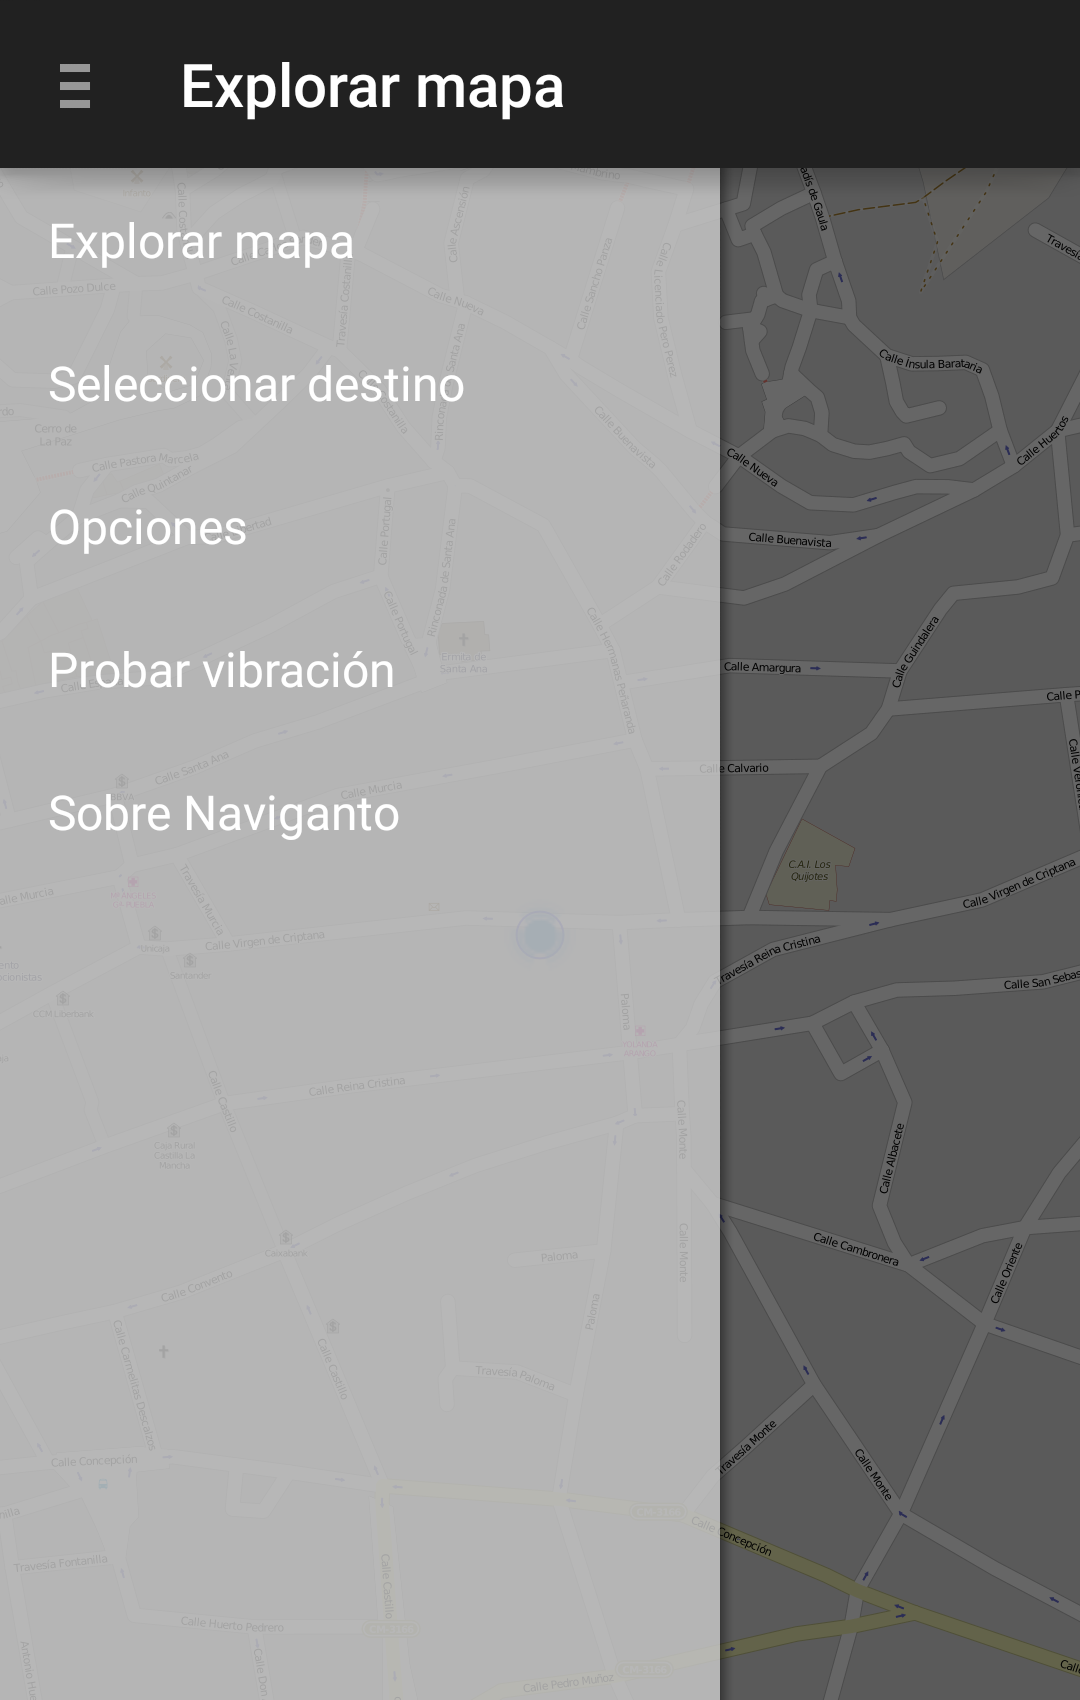
\includegraphics[width=0.85\textwidth]{/naviganto-barralateral.png}
    \end{center}
  \end{minipage}
  \begin{minipage}[b]{0.5\linewidth}
    \begin{center}
      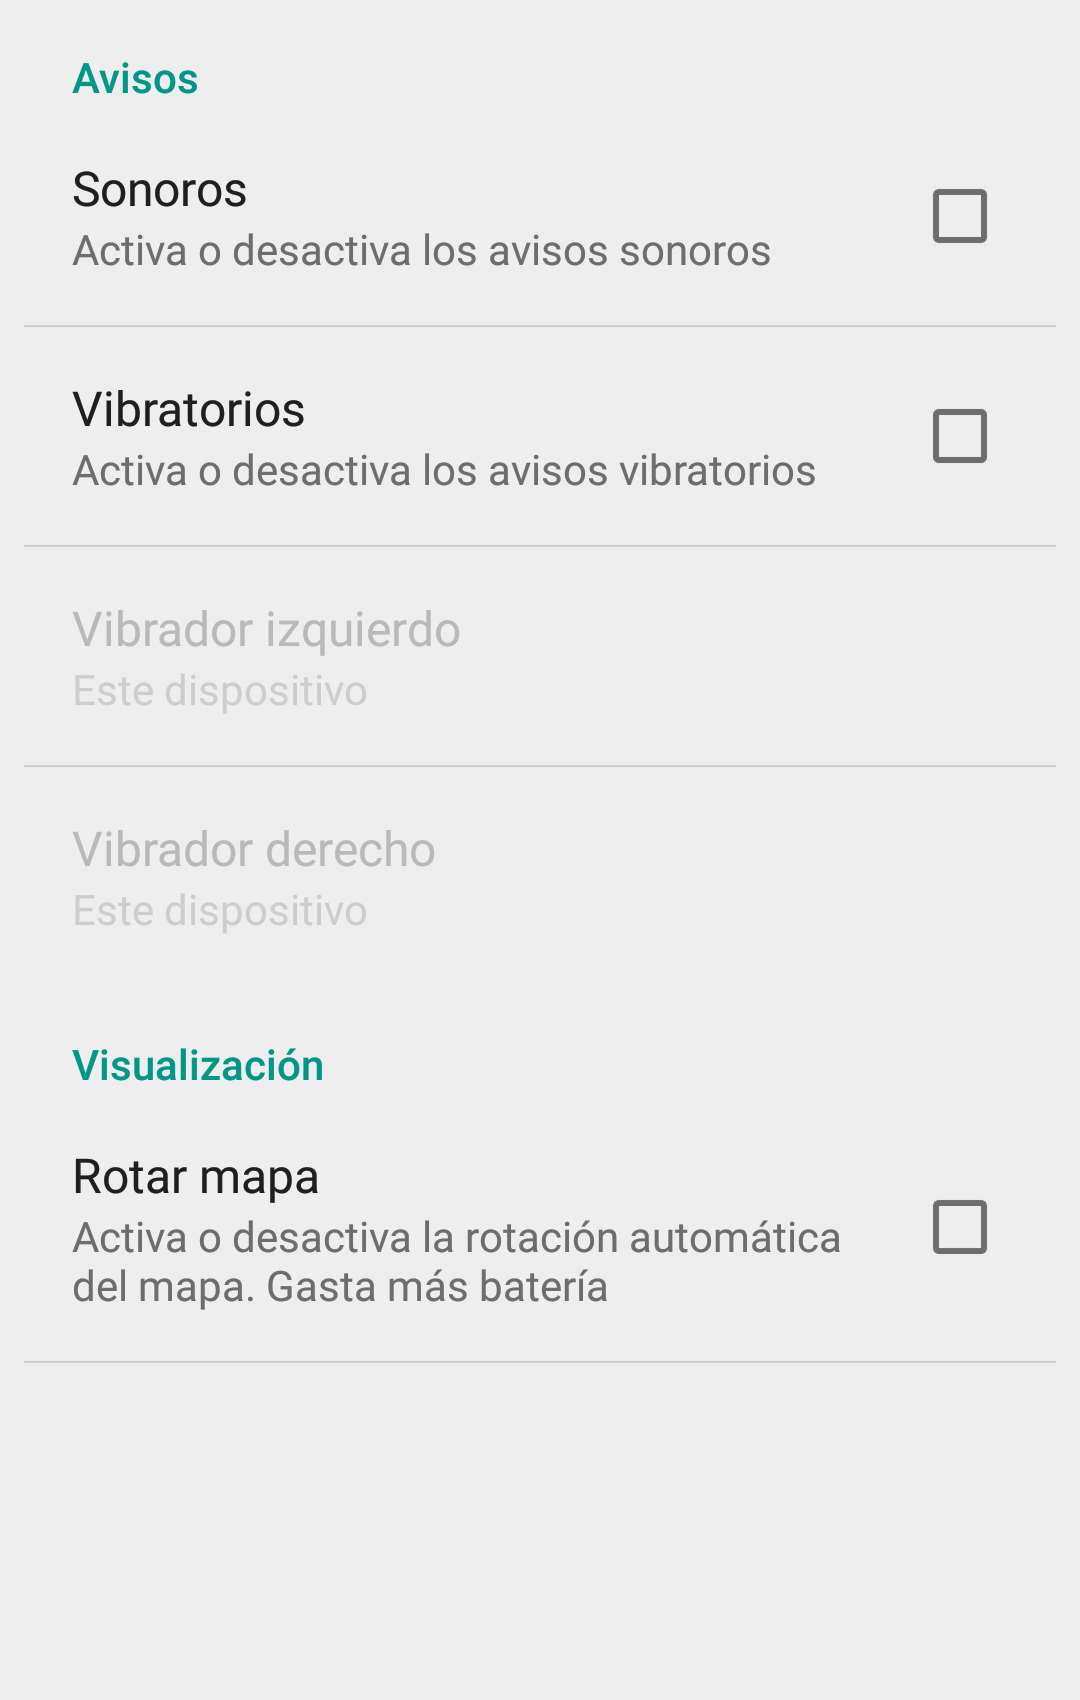
\includegraphics[width=0.85\textwidth]{/naviganto-opciones.png}
    \end{center}
  \end{minipage}
\end{figure}

Aquí podrá configurar las opciones descritas en los siguientes apartados.

\subsubsection{Avisos sonoros}

Los avisos sonoros hacen referencia a la posibilidad de escuchar cada una de las posibles
instrucciones que tengamos que realizar.

Para activar o desactivar dichos avisos basta con marcar o desmarcar la casilla del menú:

\begin{figure}[h]
  \begin{minipage}[b]{0.5\linewidth}
    \begin{center}
      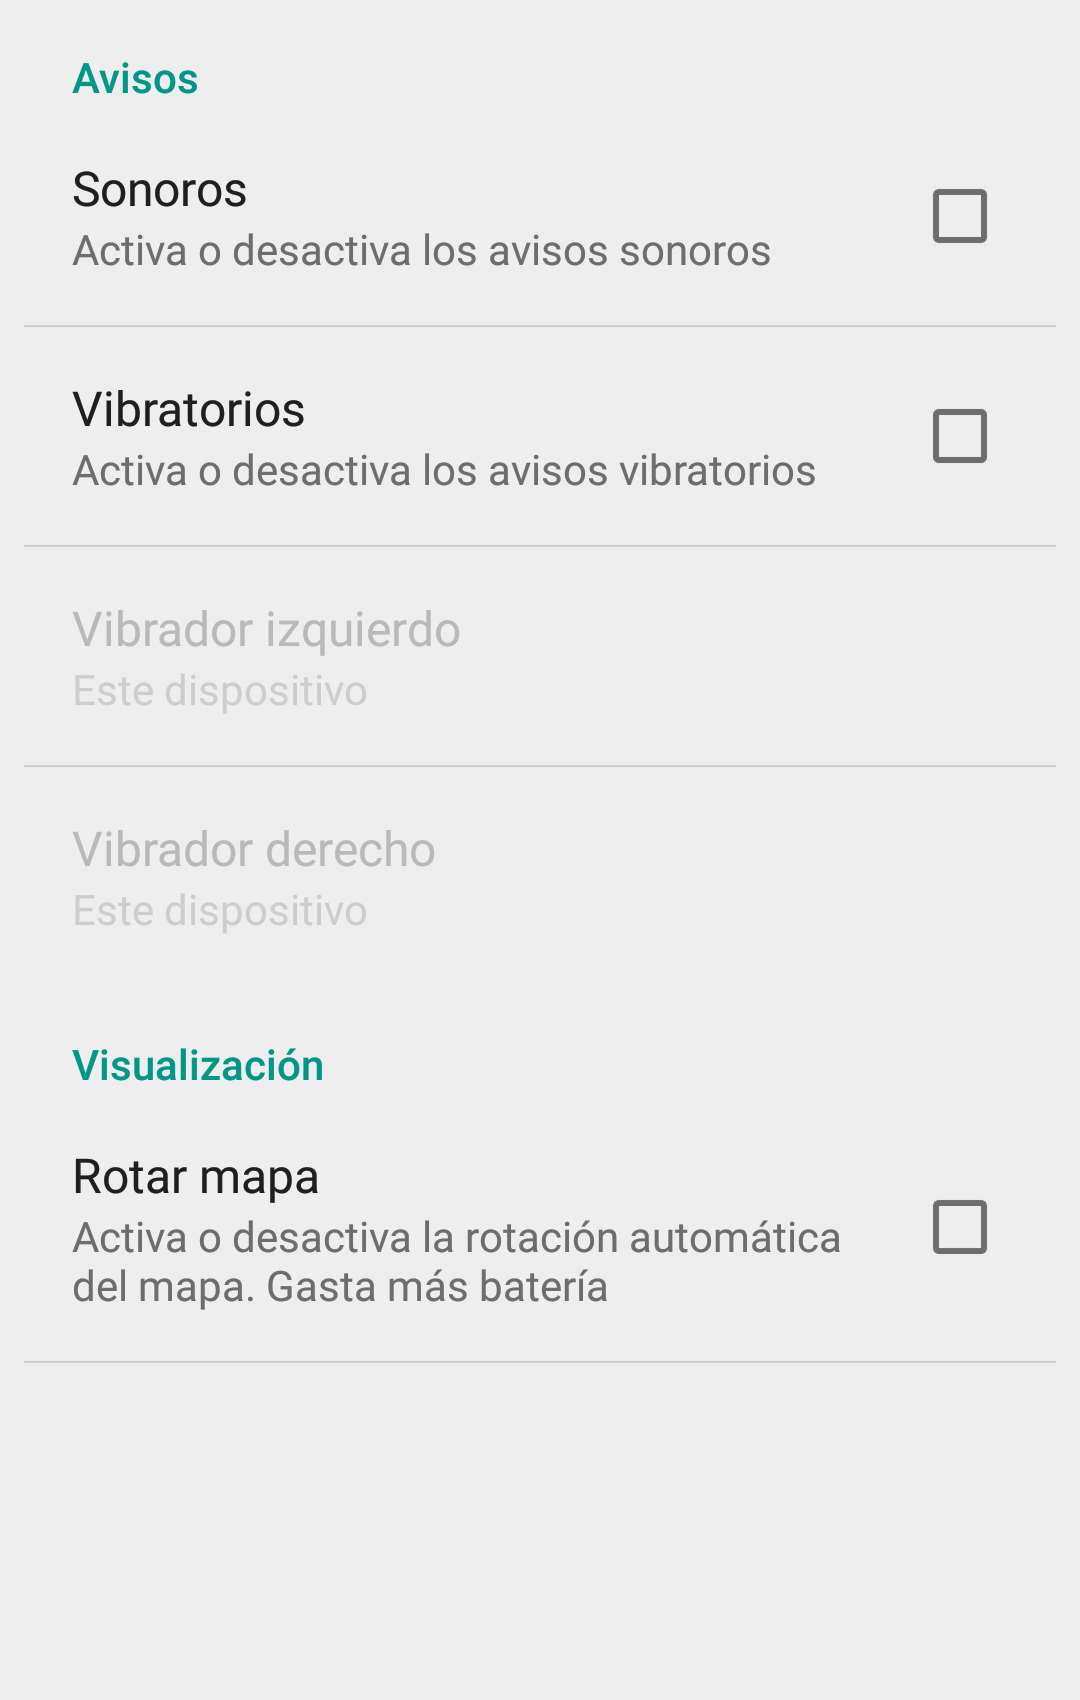
\includegraphics[width=0.85\textwidth]{/naviganto-opciones.png}
    \end{center}
  \end{minipage}
  \begin{minipage}[b]{0.5\linewidth}
    \begin{center}
      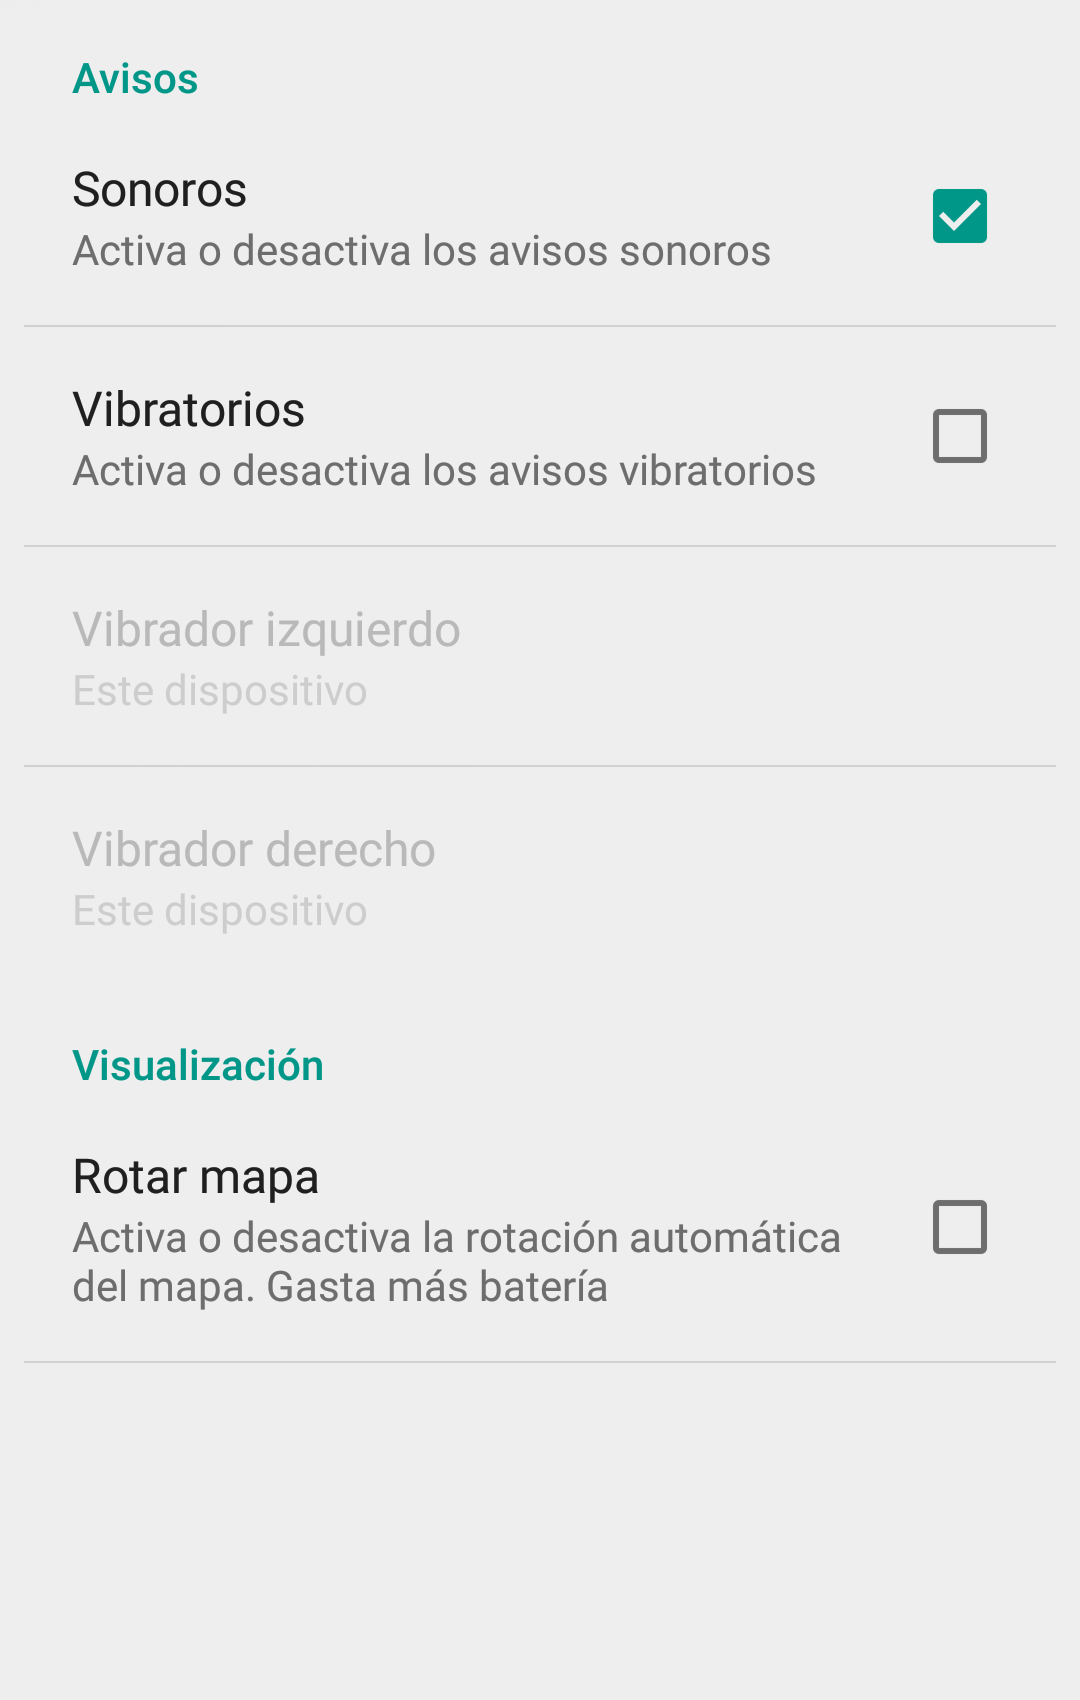
\includegraphics[width=0.85\textwidth]{/avisossonoros.png}
    \end{center}
  \end{minipage}
\end{figure}

Esta configuración se almacena en el \emph{smartphone} de forma que al cerrar y volver a abrir la
aplicación se mantenga presente.

\subsubsection{Avisos vibratorios}

Los avisos vibratorios hacen referencia a la posibilidad de que el \emph{smartphone}, junto con otro
complemento vibratorio, nos avisen de las instrucciones que tengamos que realizar.

Para activar o desactivar dichos avisos hay que activar la casilla del menú y después seleccionar
qué dispositivo colocaremos en la parte izquierda de nuestro cuerpo y cuál en la parte derecha.

\begin{figure}[h]
  \begin{minipage}[b]{0.5\linewidth}
    \begin{center}
      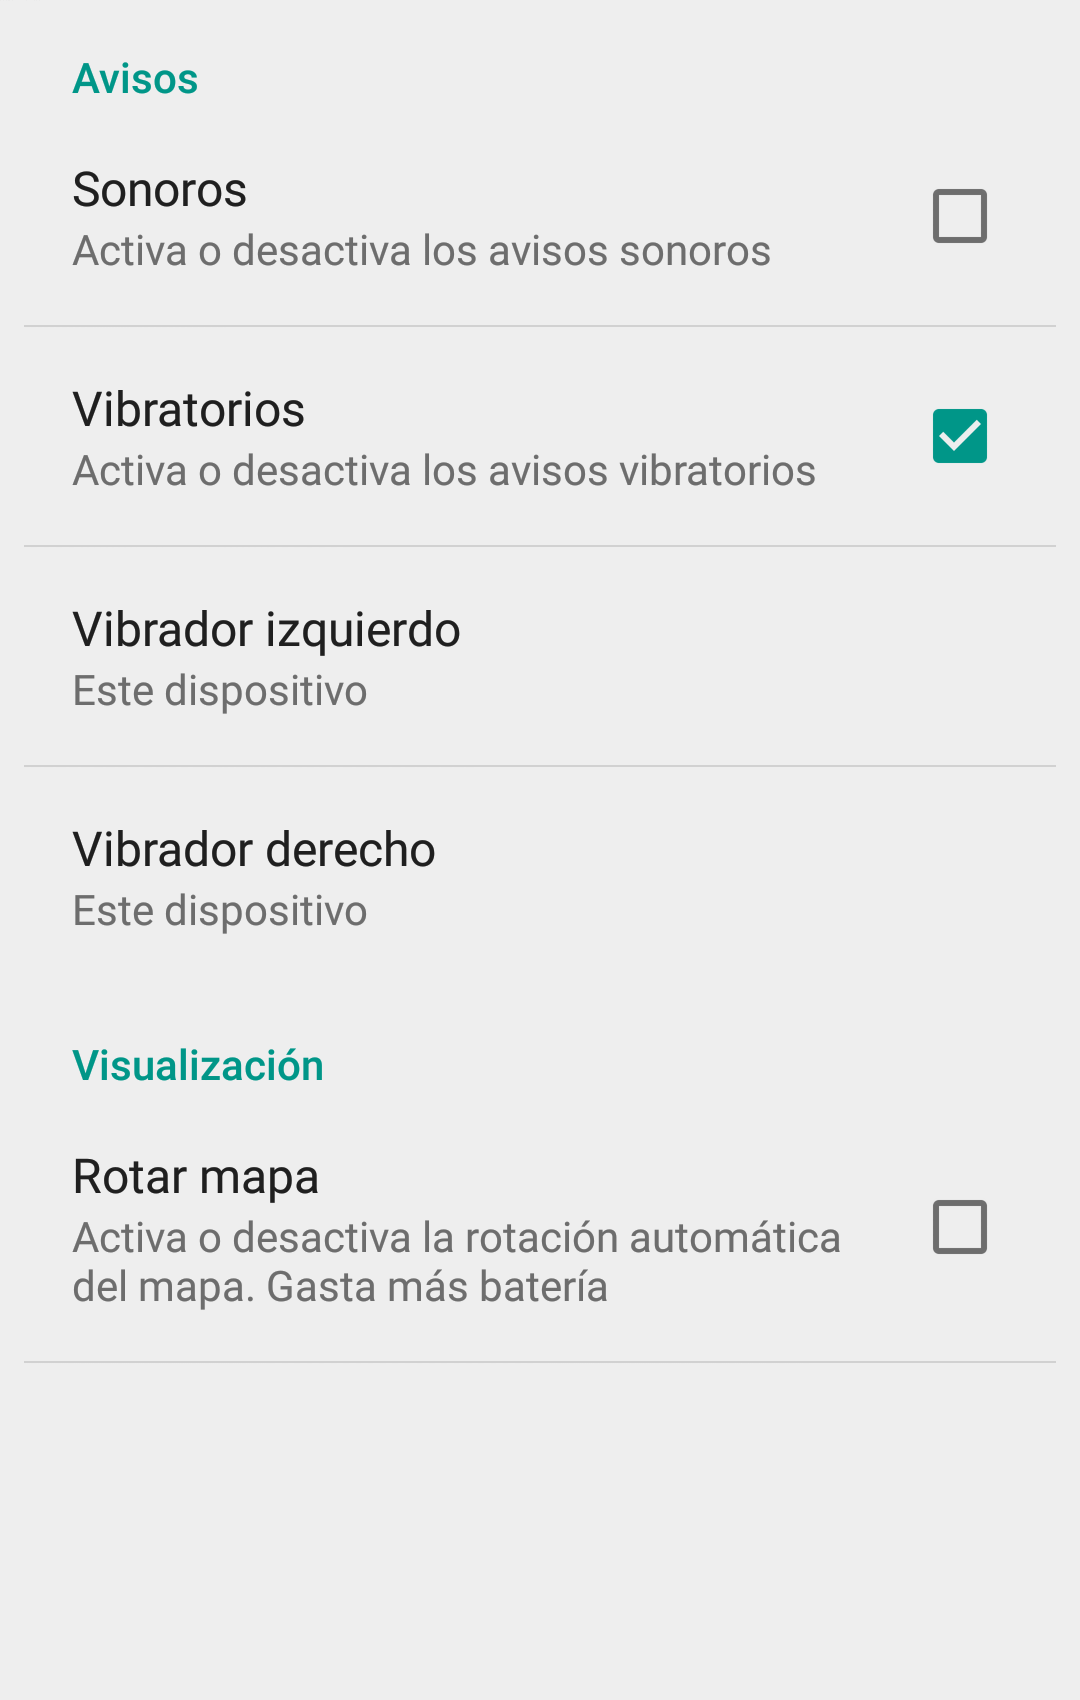
\includegraphics[width=0.76\textwidth]{/naviganto-opcionesvibrateon.png}
    \end{center}
  \end{minipage}
  \begin{minipage}[b]{0.5\linewidth}
    \begin{center}
      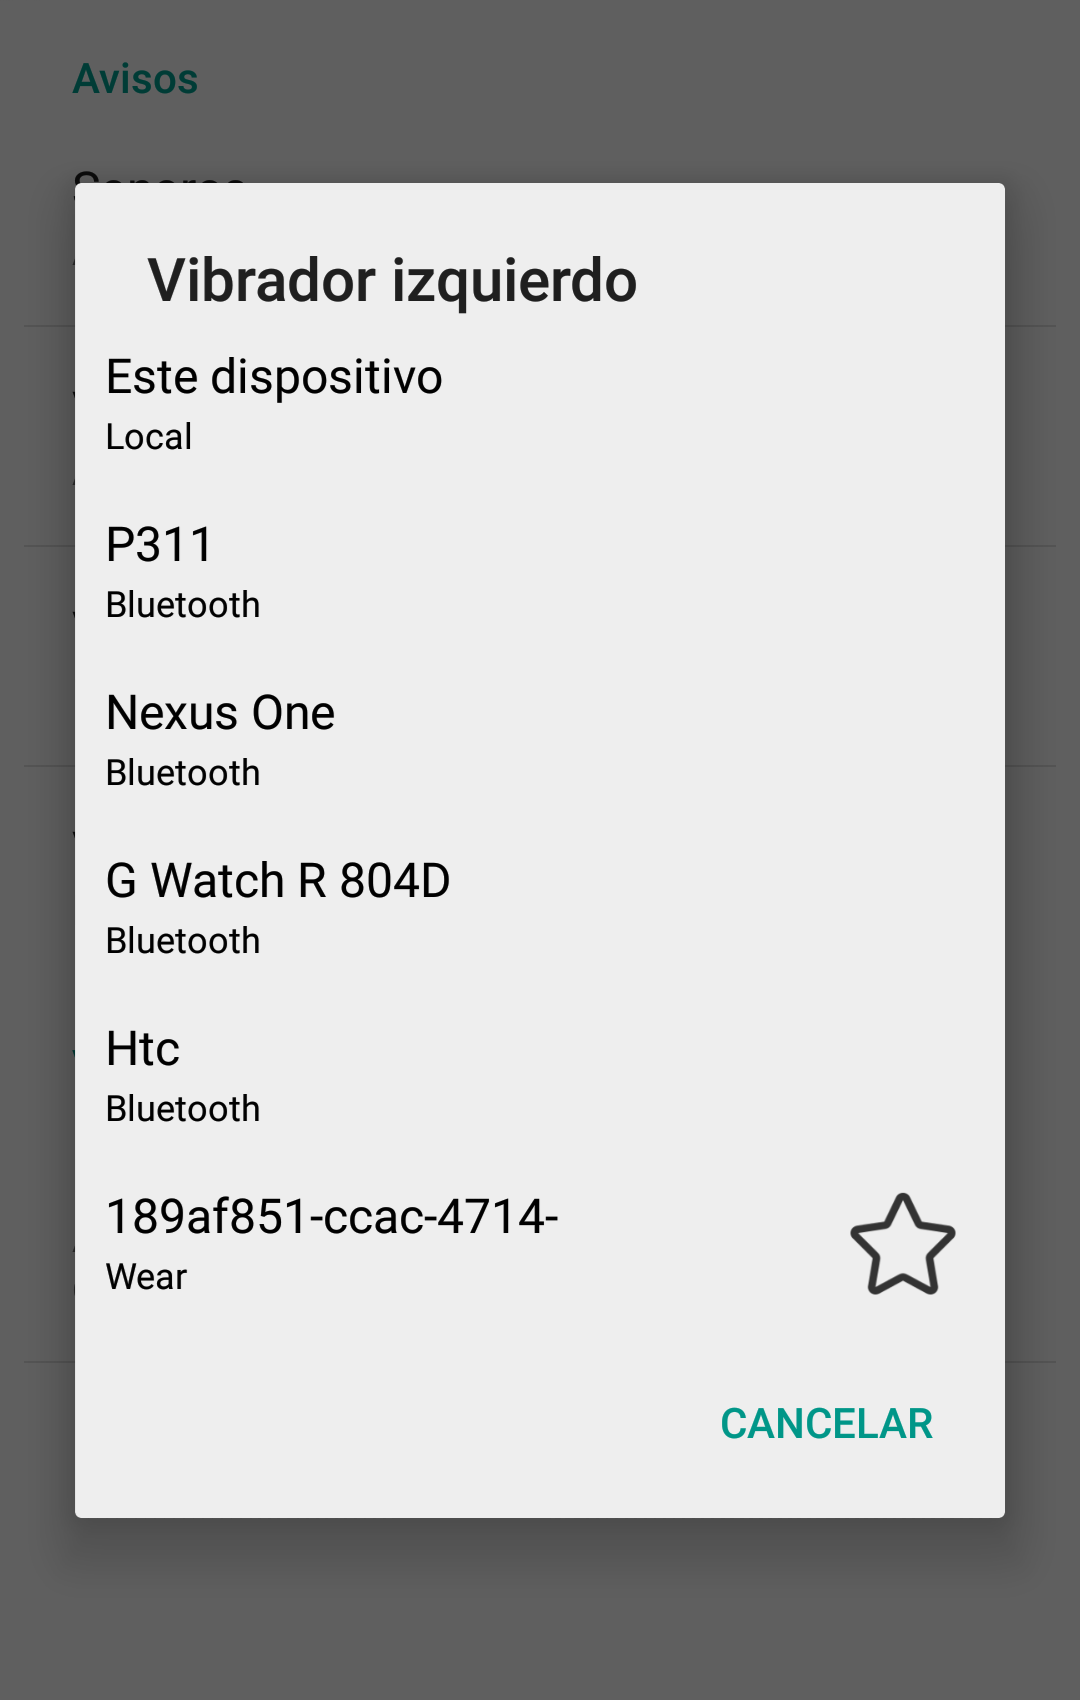
\includegraphics[width=0.76\textwidth]{/naviganto-opcioneslistadispositivos.png}
    \end{center}
  \end{minipage}
\end{figure}

Para que aparezcan dichos dispositivos en la lista debemos tener:

\begin{itemize}
  \item En caso de utilizar \textbf{Naviganto Bluetooth} como complemento, pareados los dos
    dispositivos por medio de \emph{bluetooth}.
  \item En caso de utilizar \textbf{Naviganto Wear} como complemento, sincronizado nuestro
    \emph{wearable} con el \emph{smartphone} por medio de los \emph{Play Services}.
\end{itemize}

Una vez seleccionados los dispositivos, cuando pulsemos sobre la tecla de retroceso se procederá a
la conexión con dichos dispositivos. En este punto deberán estar activas las aplicaciones en los
complementos que dispongan de \emph{Naviganto Bluetooth} y es opcional que se encuentre ejecutándose
la aplicación \emph{Naviganto Wear} en los \emph{wearables}.

\newpage
En caso de que la conexión no tenga éxito, \emph{Naviganto} nos avisará con un mensaje; en cambio,
si la conexión tiene éxito, \emph{Naviganto} nos permitirá realizar una prueba de conexión desde el
menú de la barra lateral pulsando sobre \emph{Probar vibración}.

\begin{figure}[h]
  \begin{minipage}[b]{0.5\linewidth}
    \begin{center}
      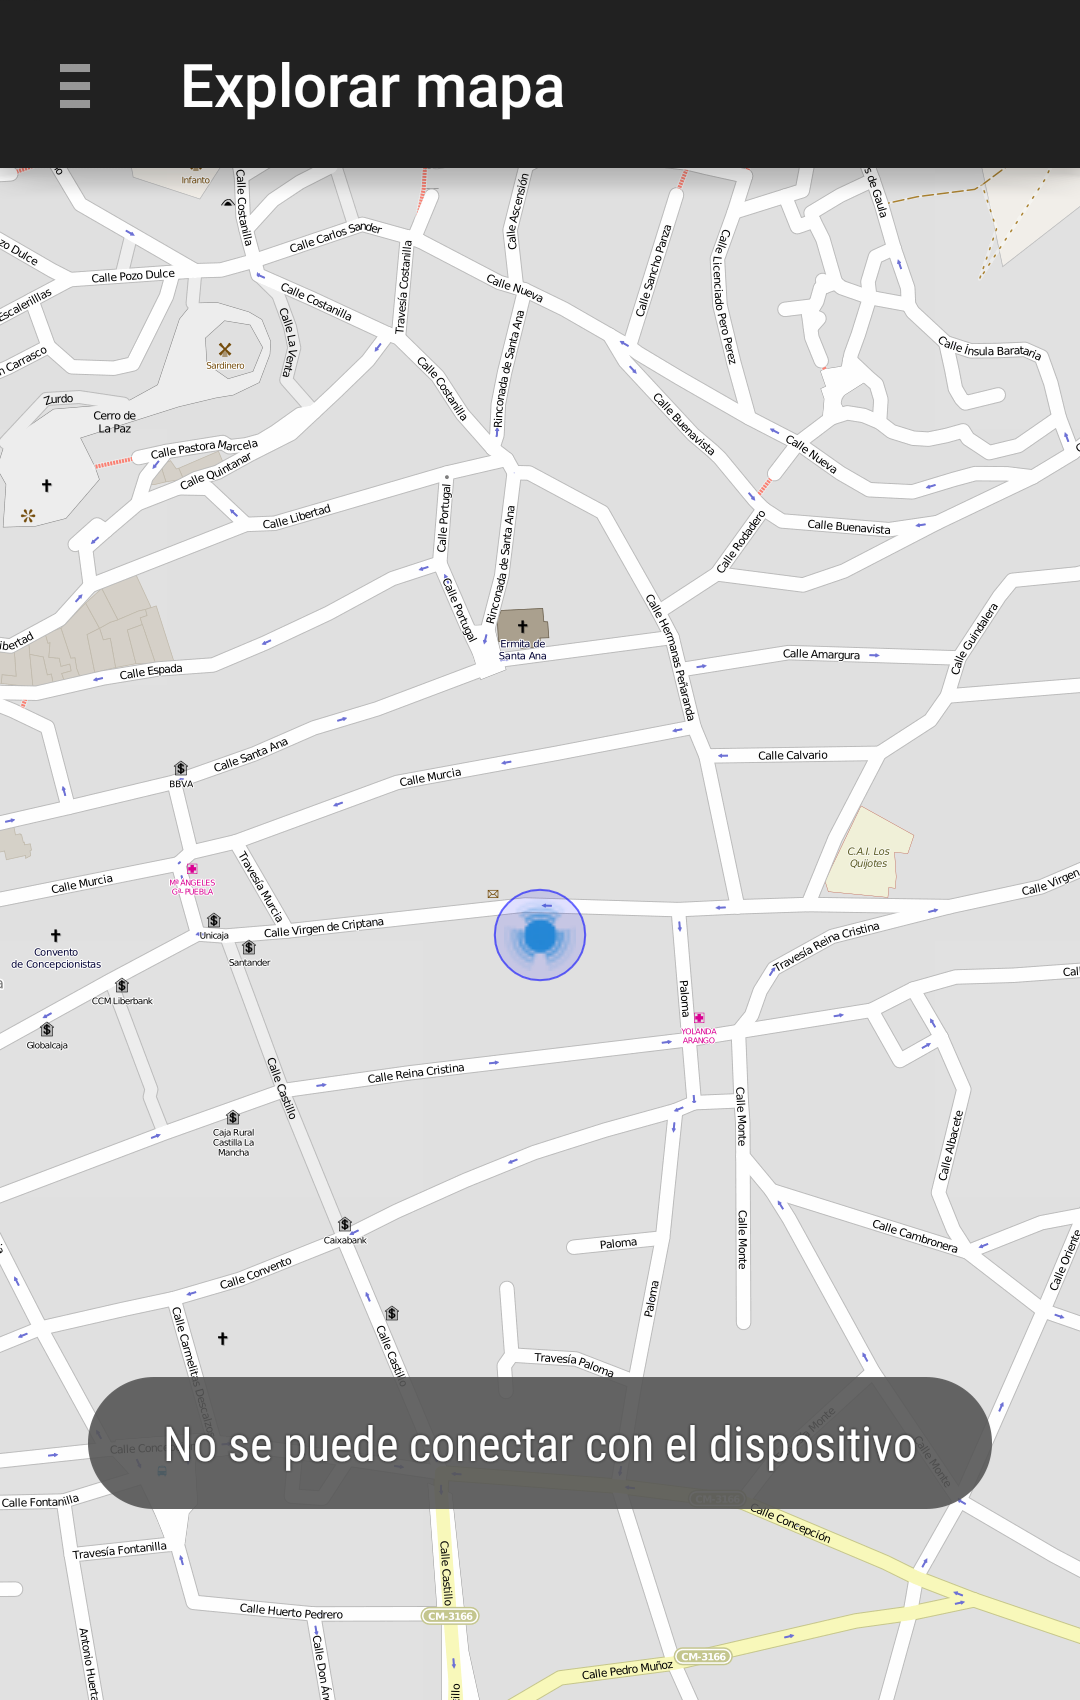
\includegraphics[width=0.76\textwidth]{/noconexiondispositivo.png}
    \end{center}
  \end{minipage}
  \begin{minipage}[b]{0.5\linewidth}
    \begin{center}
      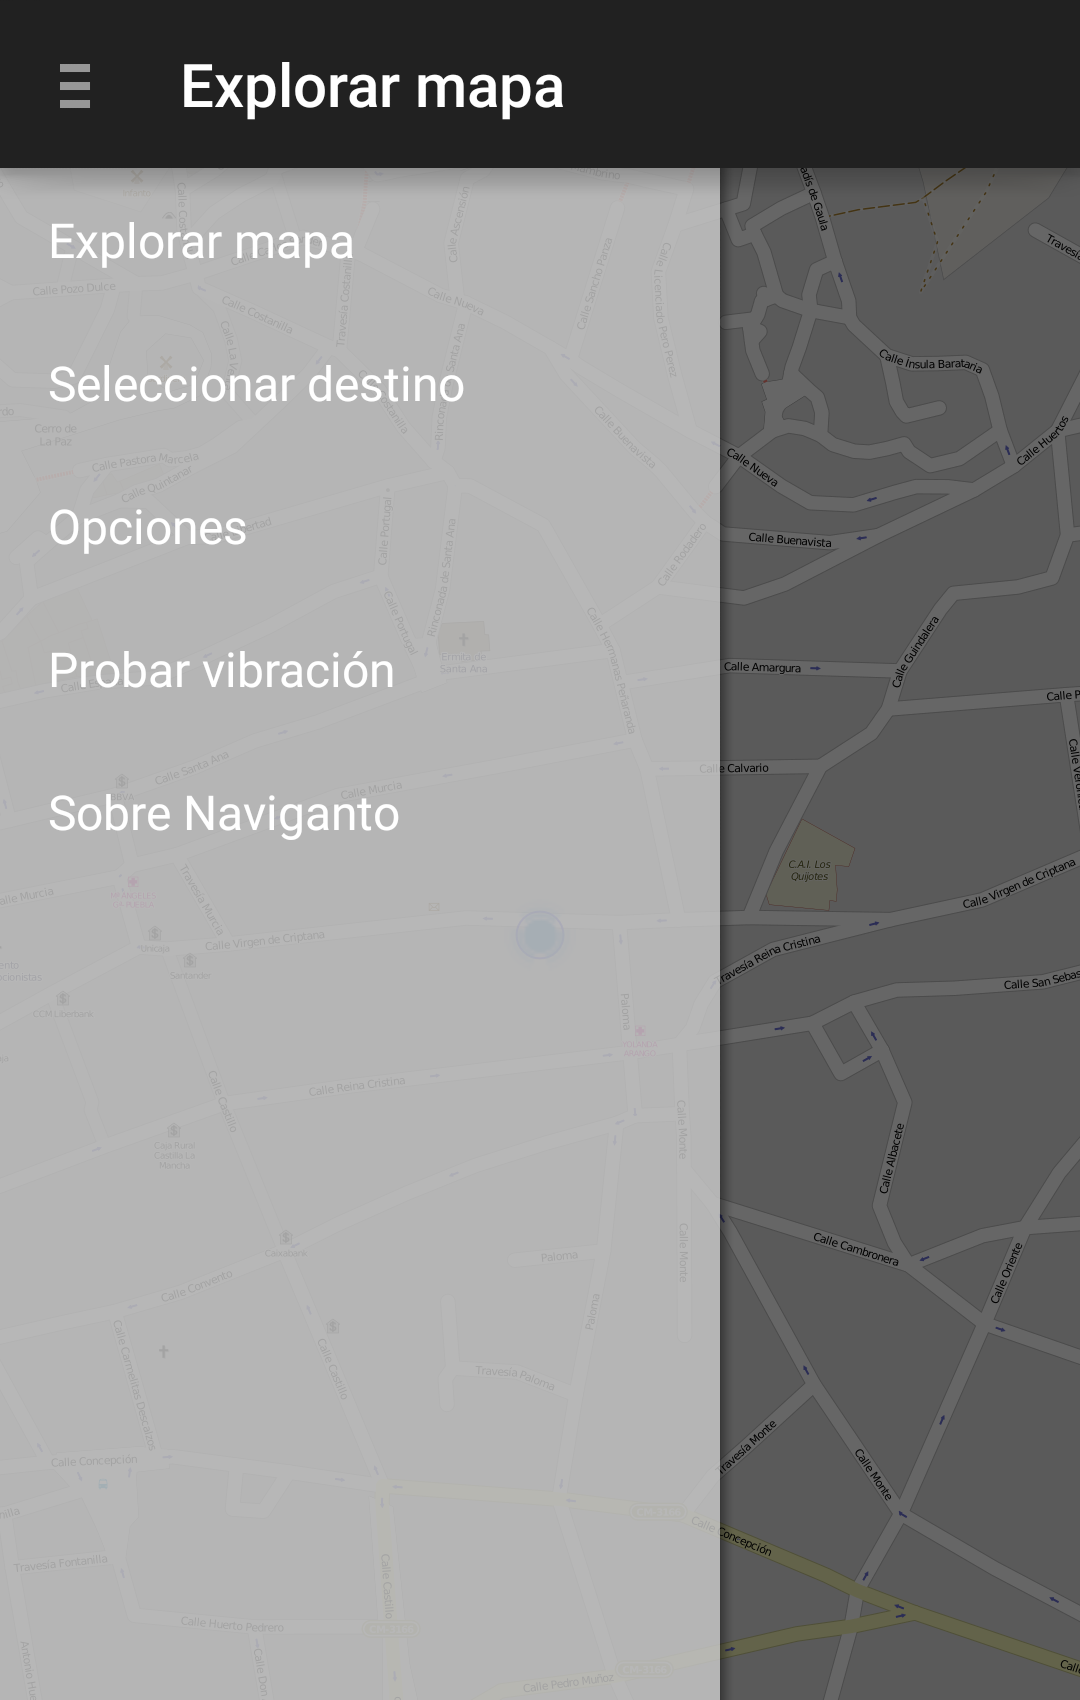
\includegraphics[width=0.76\textwidth]{/naviganto-barralateral.png}
    \end{center}
  \end{minipage}
\end{figure}

En este momento podríamos iniciar una ruta y nos guiaríamos con las vibraciones de los dispositivos,
aunque si reiniciásemos la aplicación tendríamos que volver a configurar la vibración.

\subsubsection{Rotación de mapa}

La rotación de mapa hace referencia a la posibilidad de orientar el mapa mostrado en función de la
orientación actual del \emph{smartphone}. Esta rotación conlleva un aumento considerable de uso del
procesador y, por tanto, el aumento del consumo de batería.

Para activar o desactivar esta opción basta con marcar o desmarcar la casilla del menú:

\begin{figure}[h]
  \begin{minipage}[b]{0.5\linewidth}
    \begin{center}
      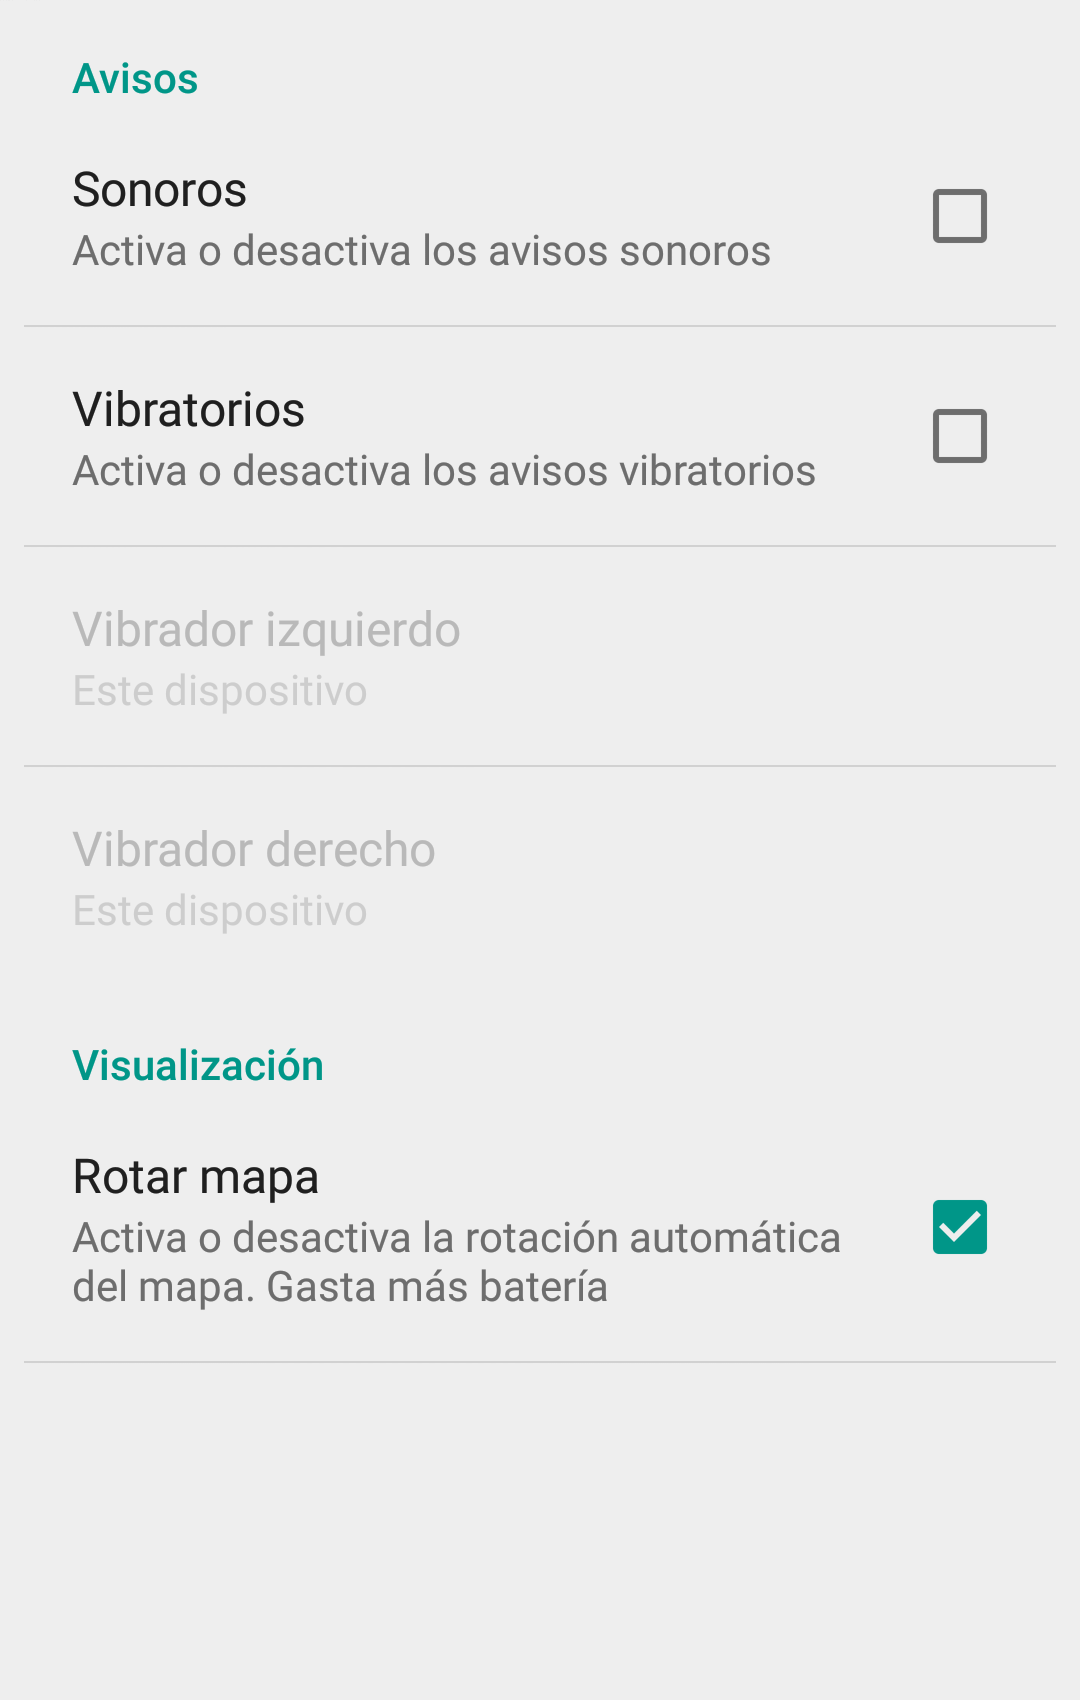
\includegraphics[width=0.85\textwidth]{/rotarmapa.png}
    \end{center}
  \end{minipage}
  \begin{minipage}[b]{0.5\linewidth}
    \begin{center}
      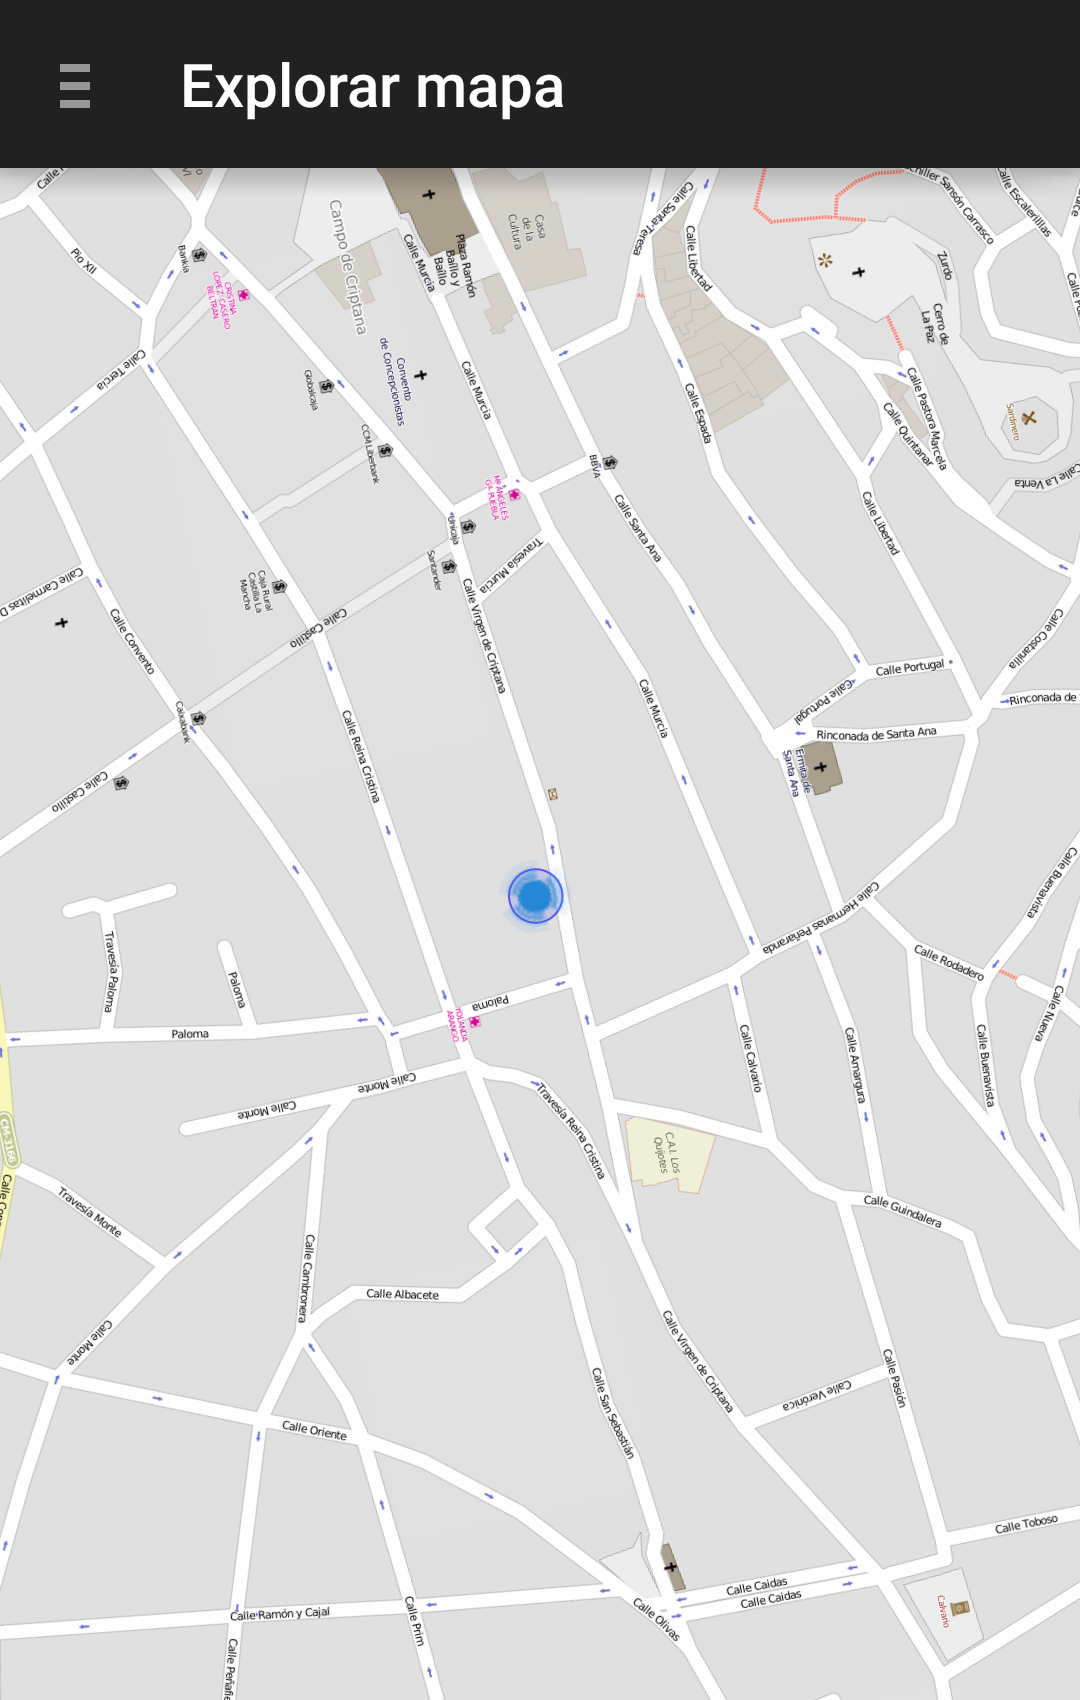
\includegraphics[width=0.85\textwidth]{/maparotado.png}
    \end{center}
  \end{minipage}
\end{figure}

Esta configuración se almacena en el \emph{smartphone} de forma que al cerrar y volver a abrir la
aplicación se mantenga presente.

\subsection{Navegación}

\subsubsection{Explorar mapa}



\subsubsection{Guiado por ruta}


\begin{figure}[h]
  \begin{minipage}[b]{0.5\linewidth}
    \begin{center}
      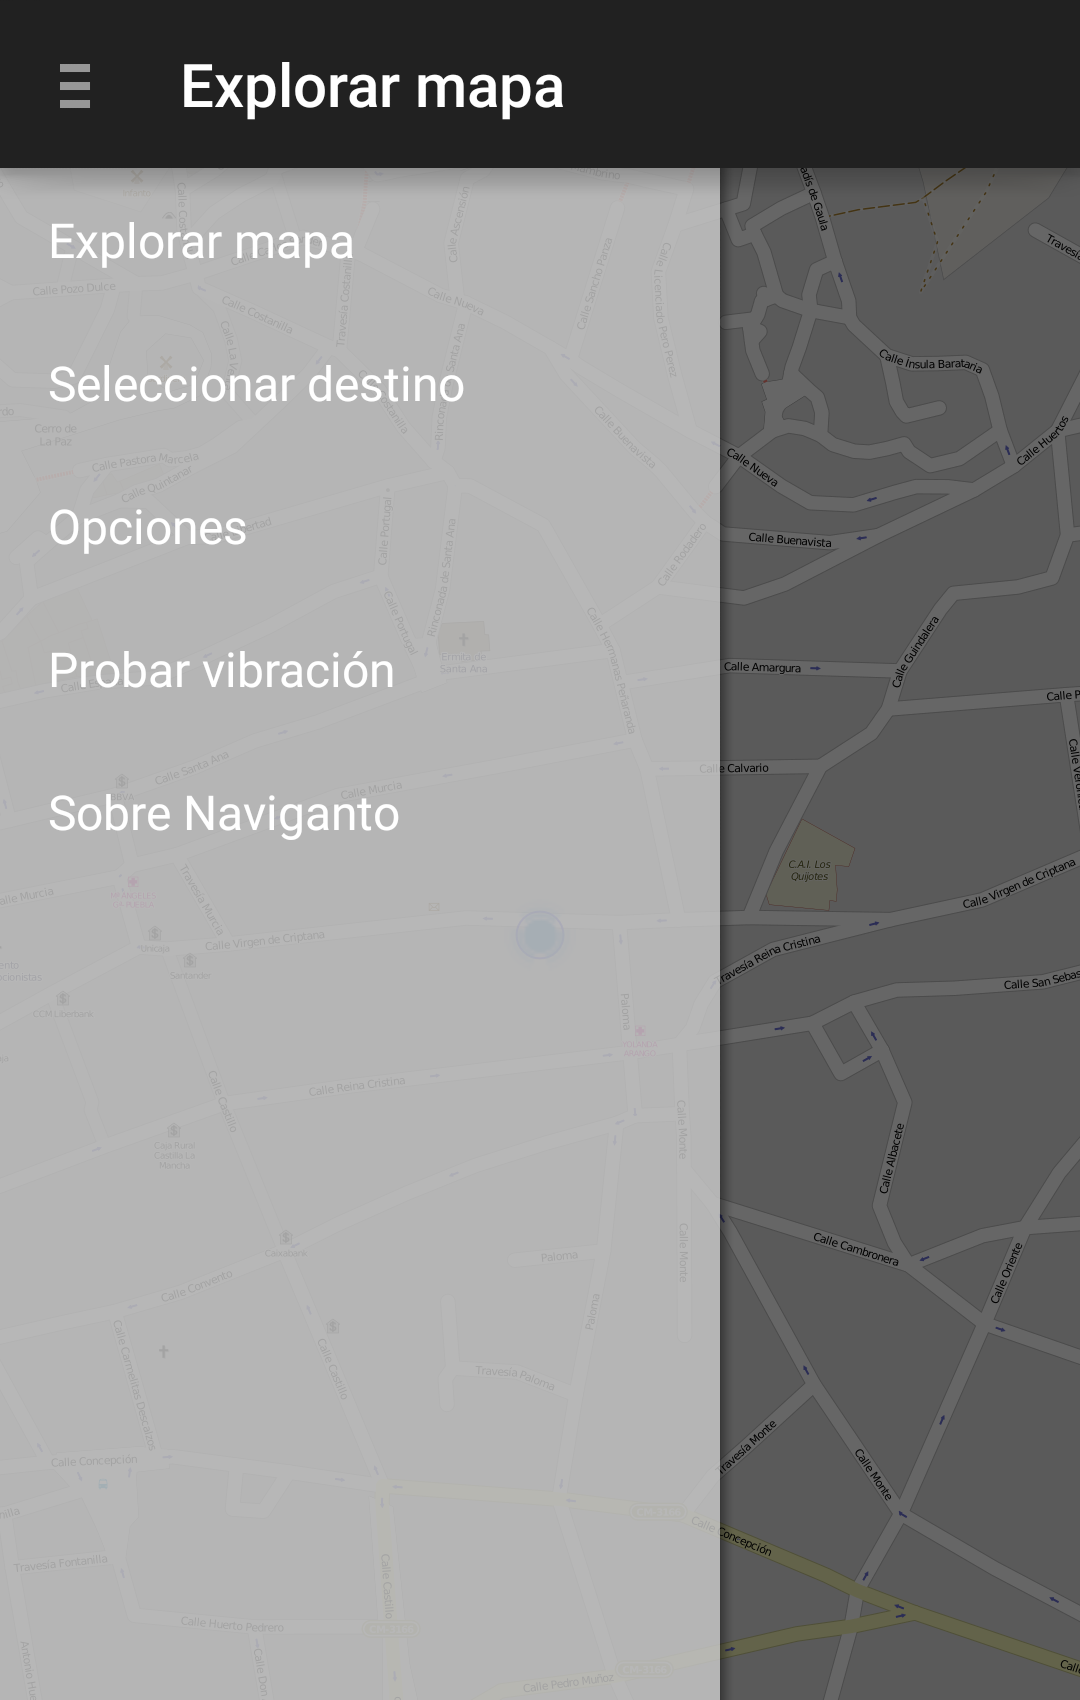
\includegraphics[width=0.85\textwidth]{/naviganto-barralateral.png}
    \end{center}
  \end{minipage}
  \begin{minipage}[b]{0.5\linewidth}
    \begin{center}
      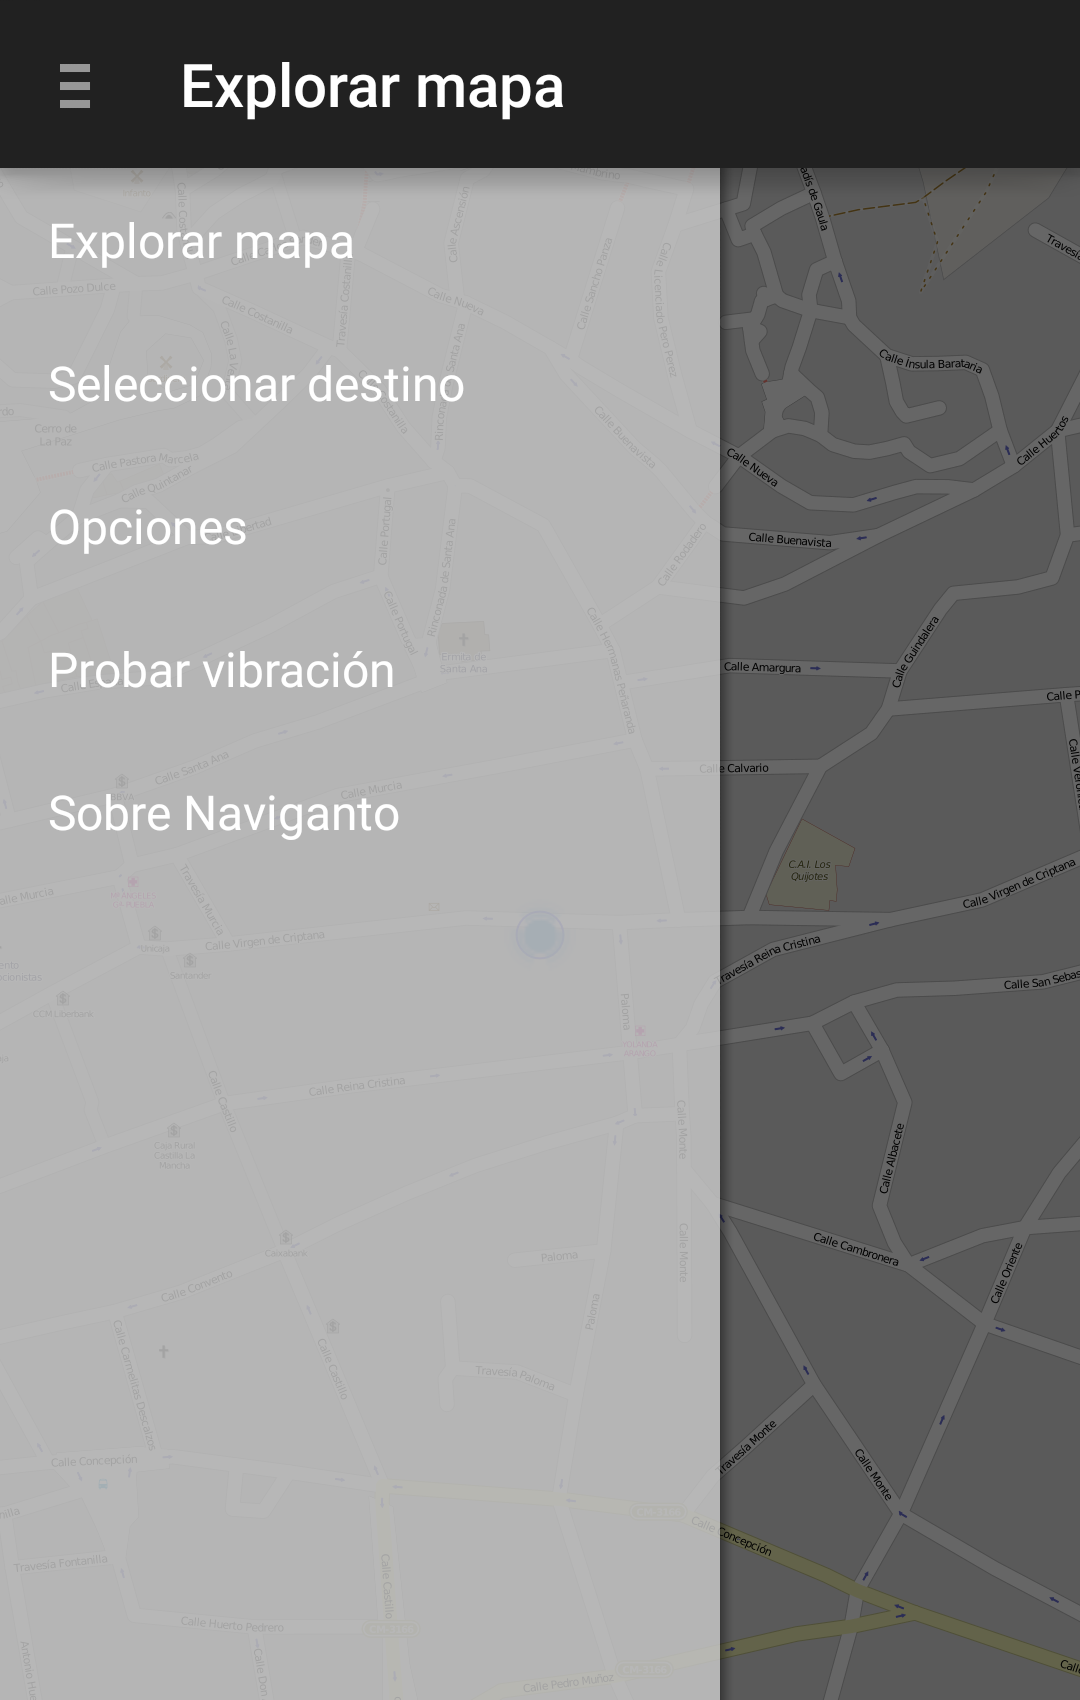
\includegraphics[width=0.85\textwidth]{/naviganto-barralateral.png}
    \end{center}
  \end{minipage}
\end{figure}

\begin{figure}[h]
  \begin{center}
    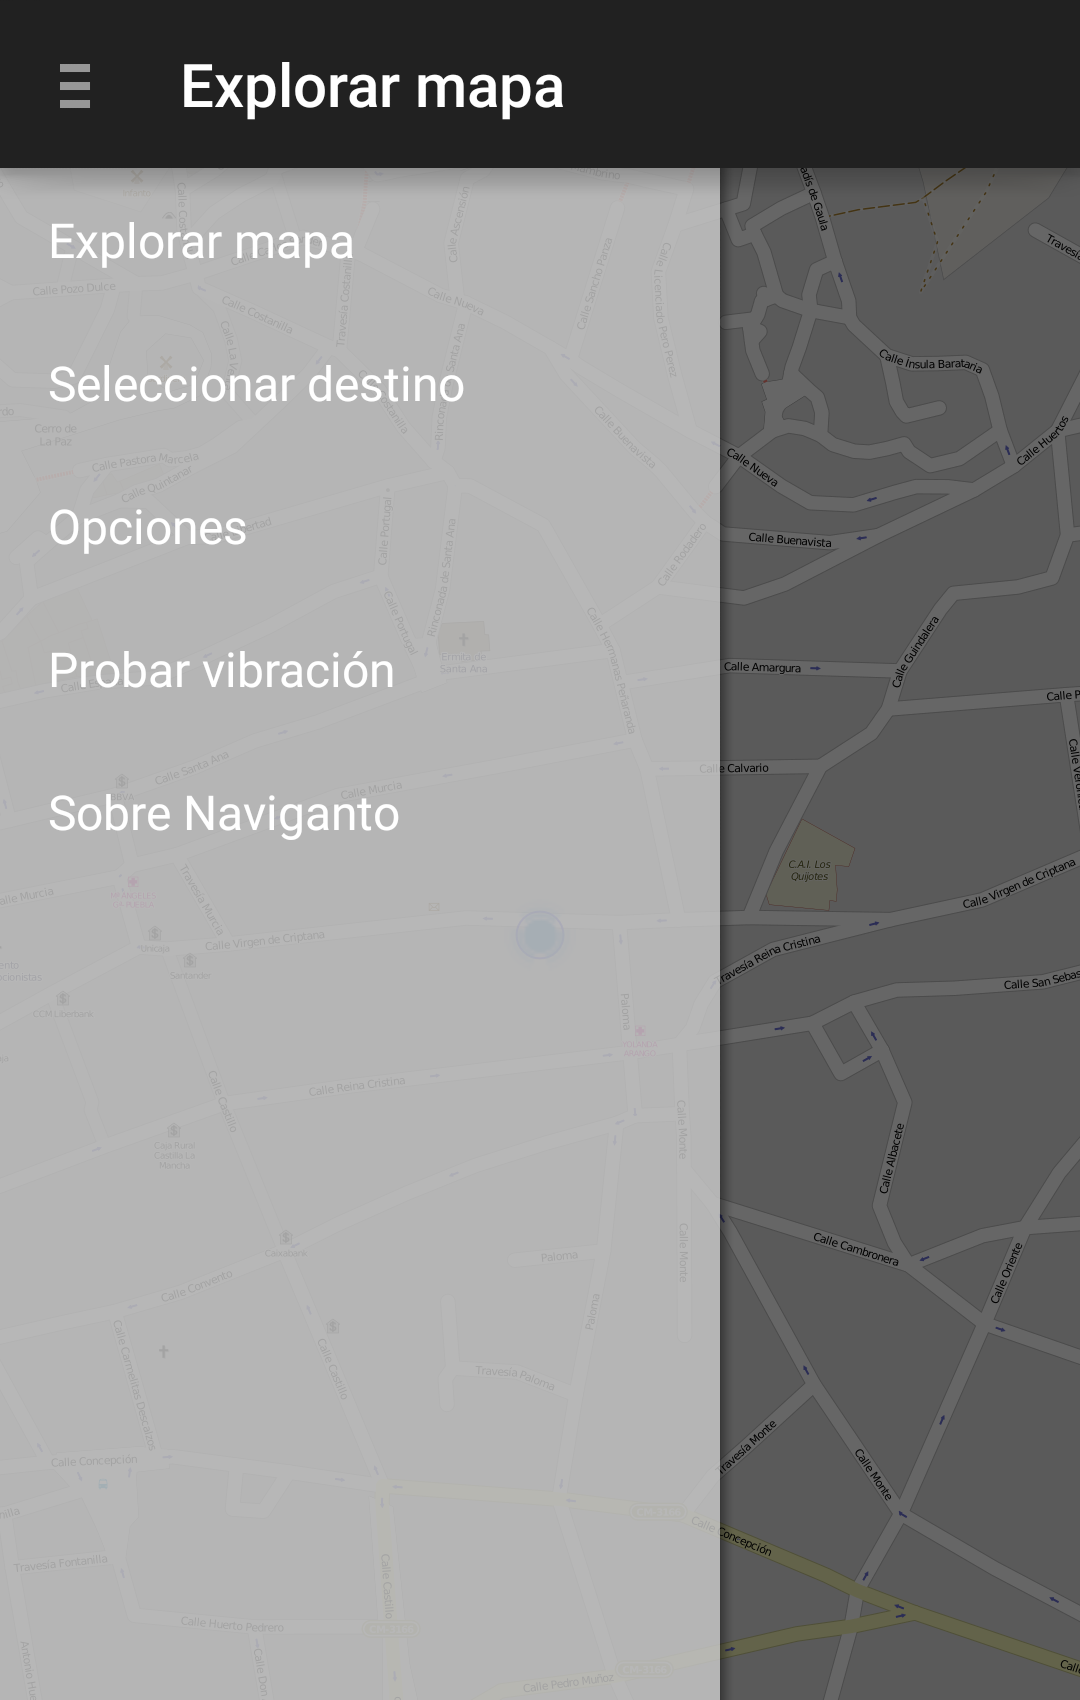
\includegraphics[width=0.425\textwidth]{/naviganto-barralateral.png}
  \end{center}
\end{figure}

% Local Variables:
% TeX-master: "main.tex"
%  coding: utf-8
%  mode: latex
%  mode: flyspell
%  ispell-local-dictionary: "castellano8"
% End:
